\documentclass{article}

\usepackage{graphicx}
\graphicspath{ {./images/} }

\title{Ch. 36 Solutions}
\author{Principles of Macroeconomics}
\date{\today}

\begin{document}

\maketitle

\section*{Problems and Applications}

\begin{enumerate}

\item \phantom{x}

	\begin{center}
	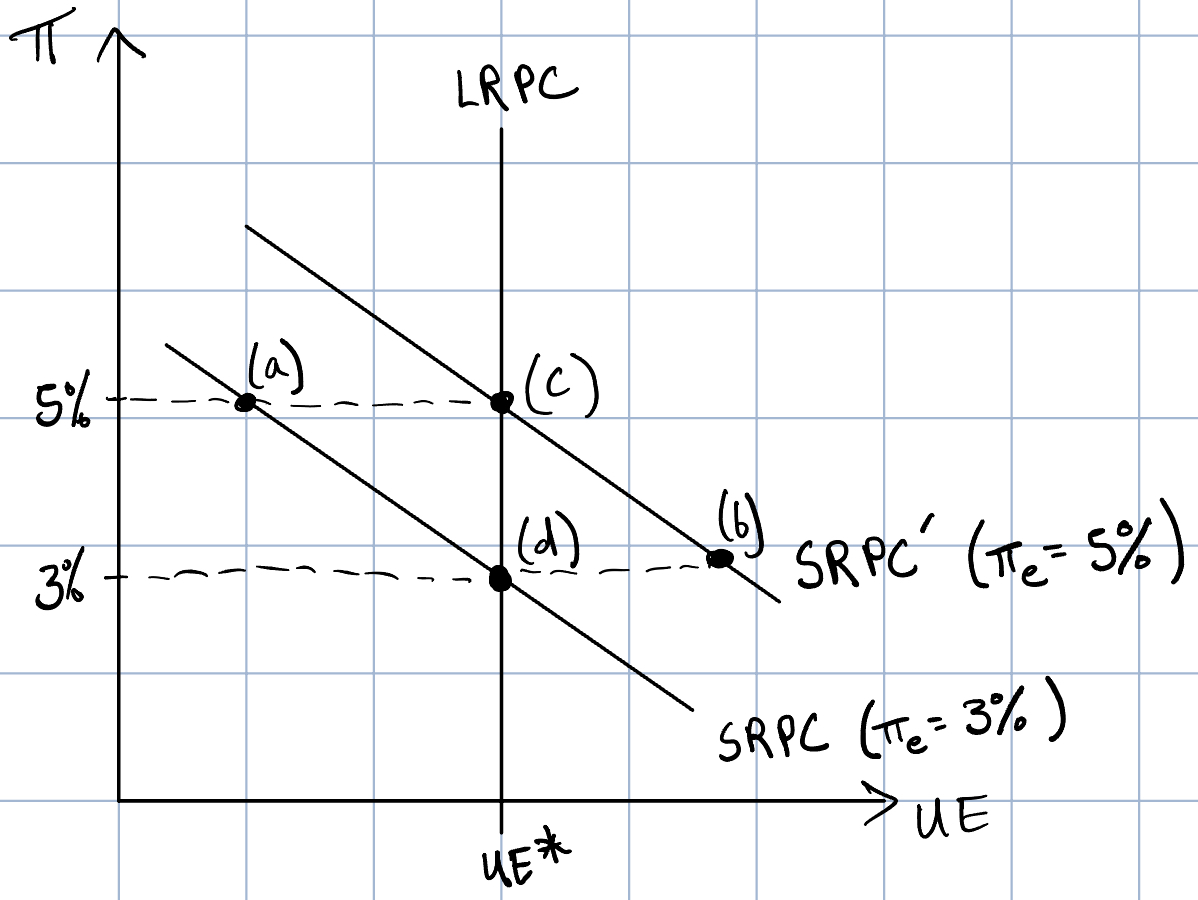
\includegraphics[width = 0.5\textwidth]{paa1}
	\end{center}

\item

	\begin{enumerate}
	
	\item If the natural rate of unemployment increases, the long-run Phillips curve shifts right because the long run Phillips curve is vertical at the natural rate of unemployment. Typically, a development that increases the natural rate of unemployment will shift LRAS and SRAS to the left. That's because a higher unemployment rate means fewer people are working, and when fewer people are working, the economy produces less. When SRAS shifts left, it causes the short-run Phillips curve to shift right.
	
		\begin{center}
		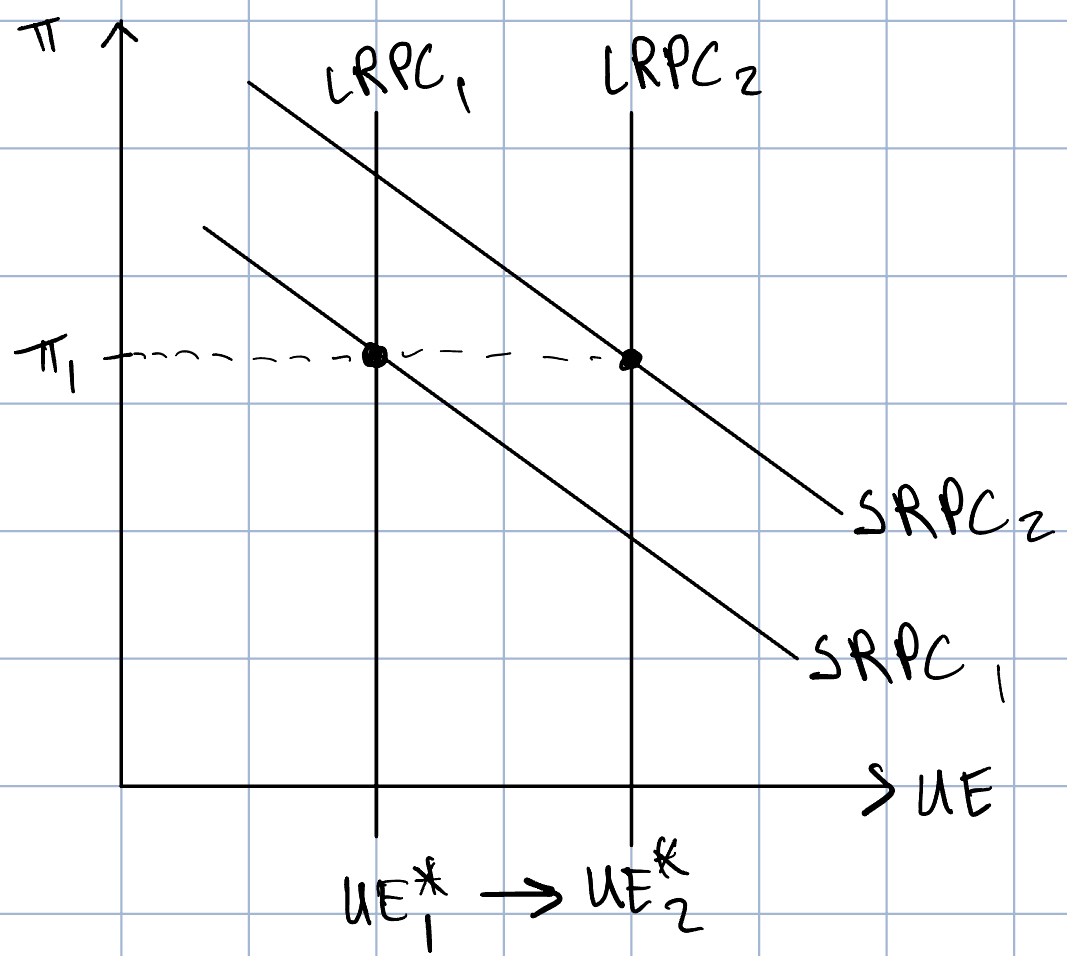
\includegraphics[width = 0.4\textwidth]{paa2a}
		\end{center}
	
	\item A decline in the price of oil is a positive supply shock, so the SRAS curve shifts to the right. In response to a positive supply shock, the short-run Phillips curve shifts left. 
	
		\begin{center}
		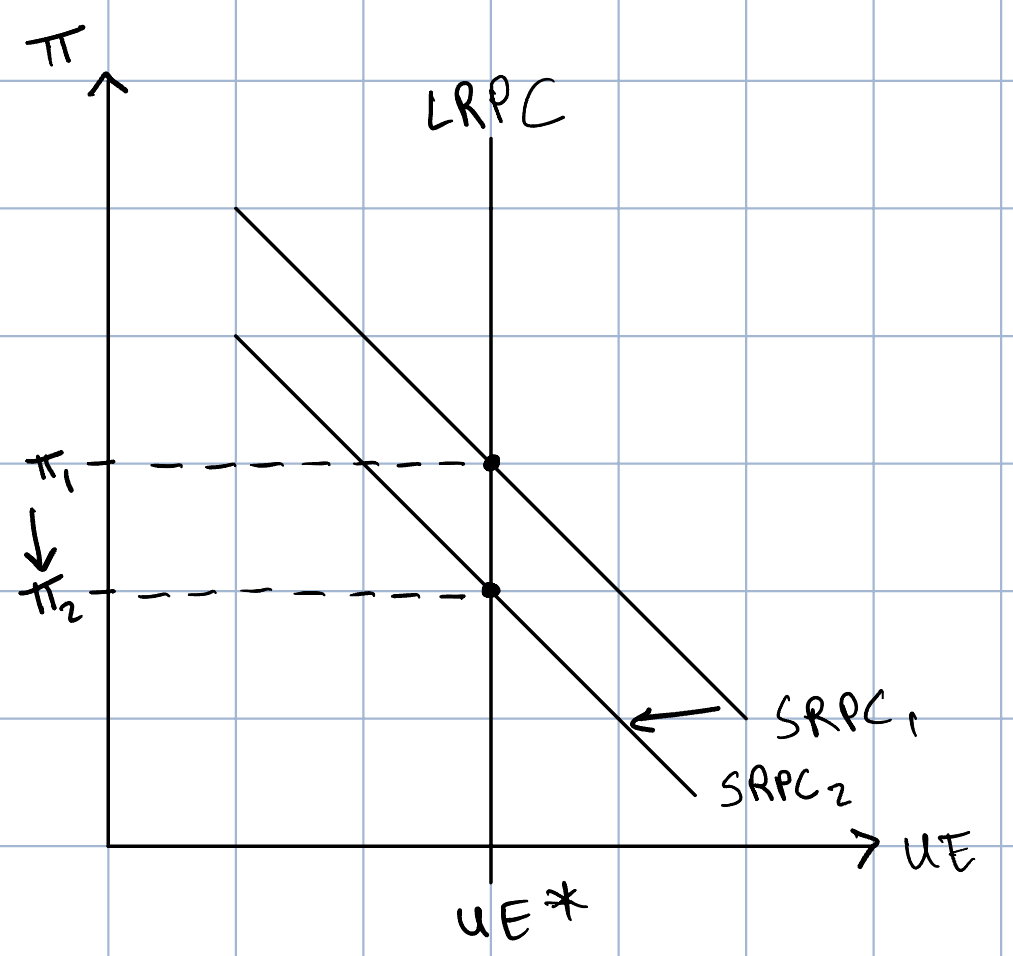
\includegraphics[width = 0.4\textwidth]{paa2b}
		\end{center}
	
	\item A rise in government spending shifts the AD curve to the right. That decreases unemployment and increases inflation, so there's a movement up and to the left along the short-run Phillips curve.
	
		\begin{center}
		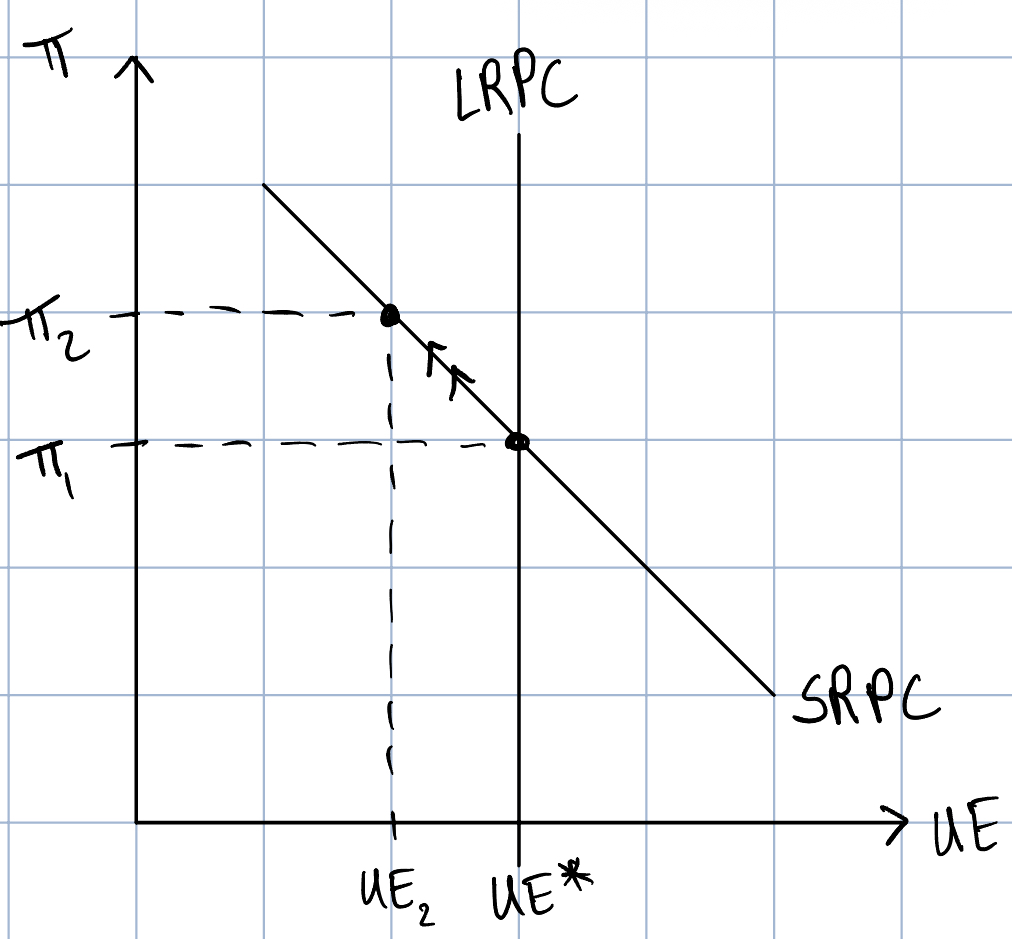
\includegraphics[width = 0.4\textwidth]{paa2c}
		\end{center}
	
	\item When expected inflation declines, the SRAS curve shifts to the right. That causes the short-run Phillips curve to shift to the left. 
	
		\begin{center}
		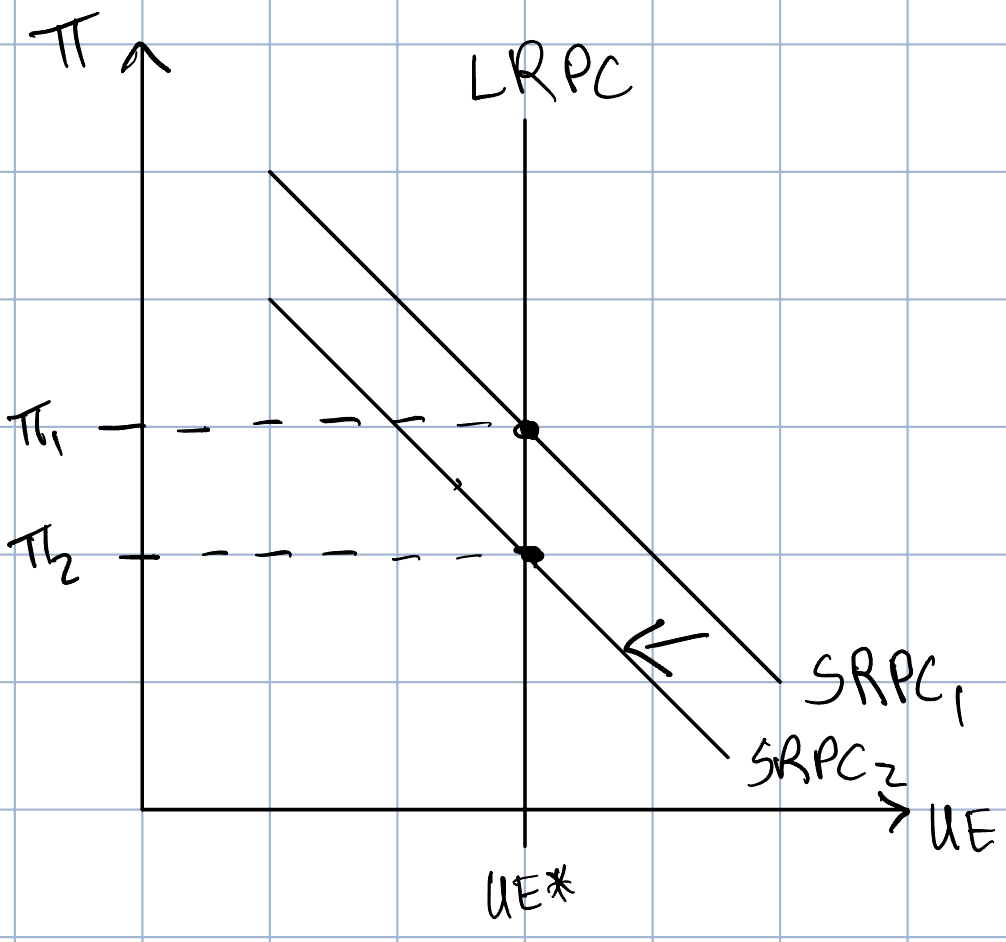
\includegraphics[width = 0.4\textwidth]{paa2d}
		\end{center}
	
	\end{enumerate}
	
\newpage
	
\item

	\begin{enumerate}
	
	\item In the short run, inflation decreases and unemployment increases.
	
		\begin{center}
		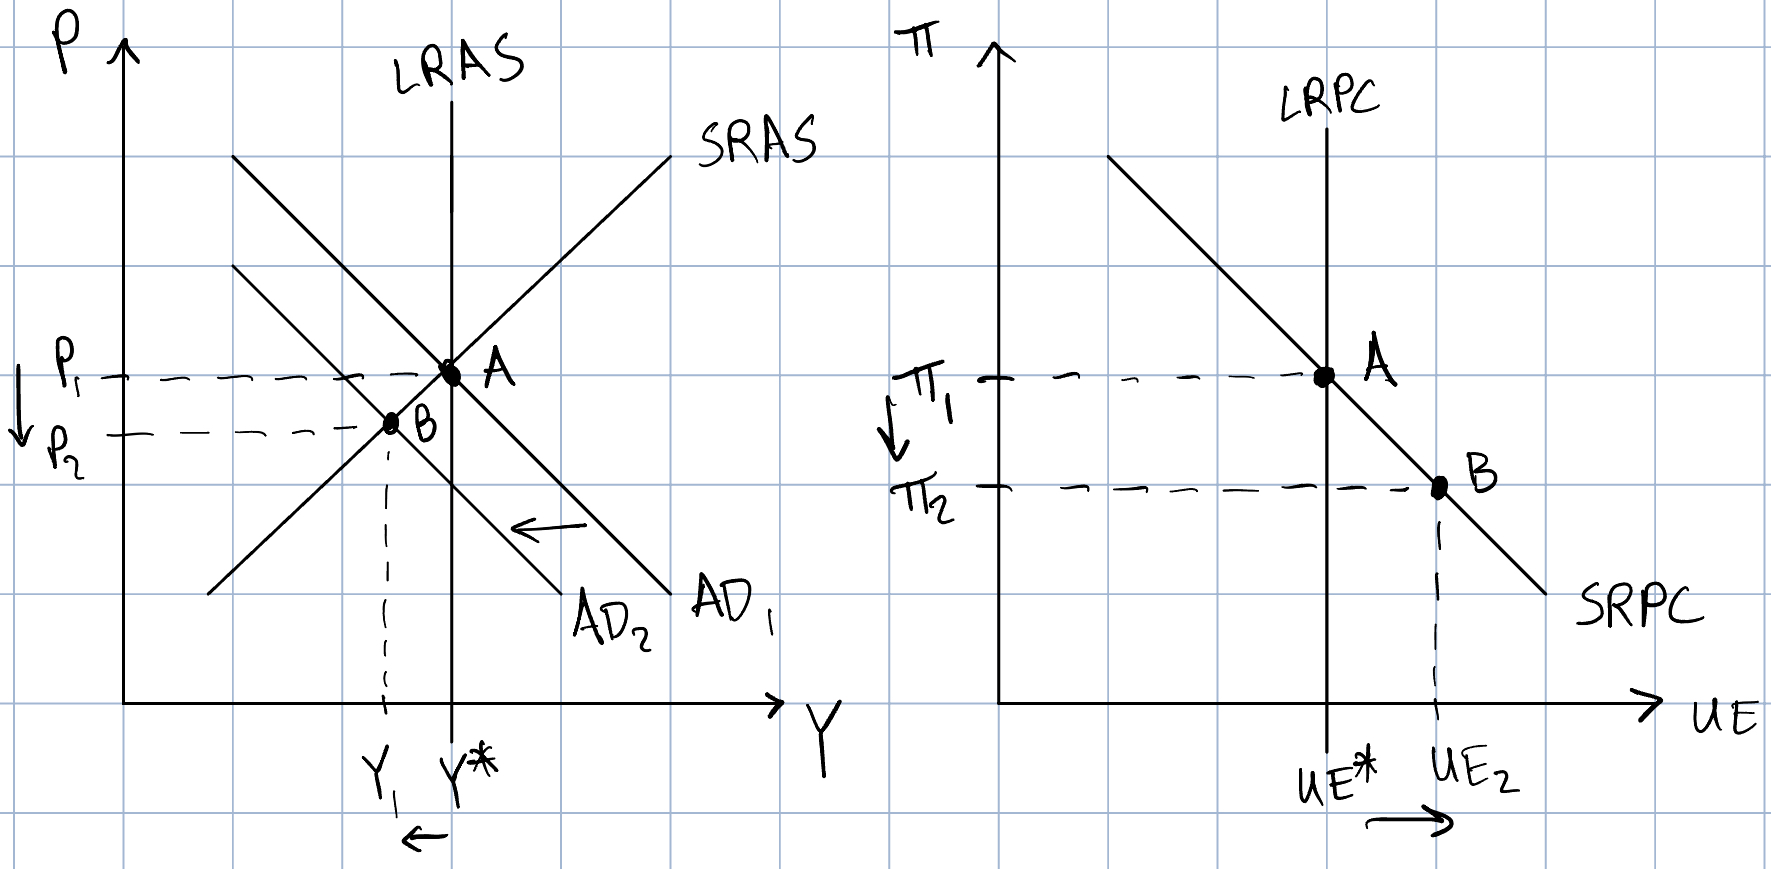
\includegraphics[width = \textwidth]{paa3a}
		\end{center}
	
	\item If expected inflation decreases, then the short-run Phillips curve will shift to the left. After the recession, the economy faces a better set of inflation-unemployment combinations because for any given level of unemployment, the corresponding inflation rate is now lower. 
	
		\begin{center}
		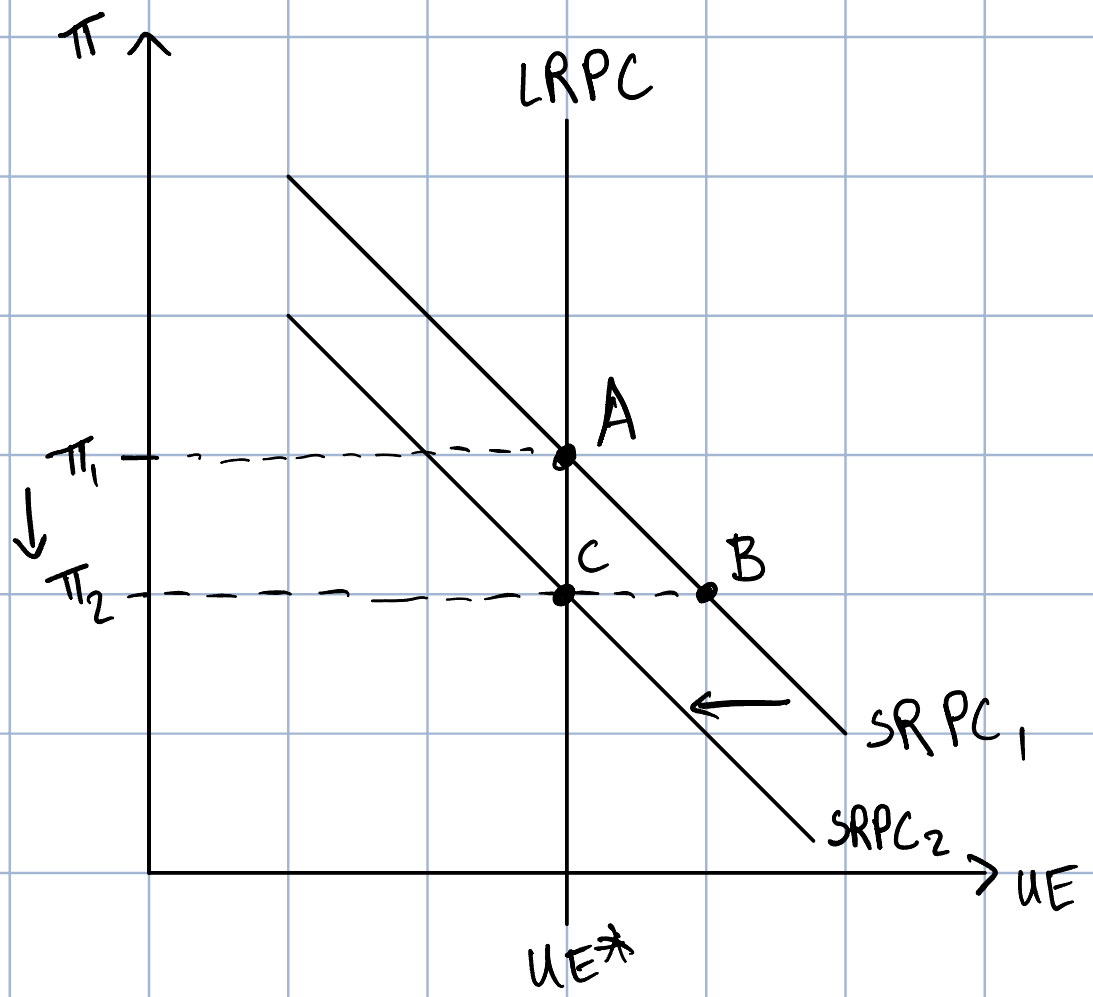
\includegraphics[width = 0.4\textwidth]{paa3b}
		\end{center}
	
	\end{enumerate}
	
\item

	\begin{enumerate}
	
	\item \phantom{x}
	
		\begin{center}
		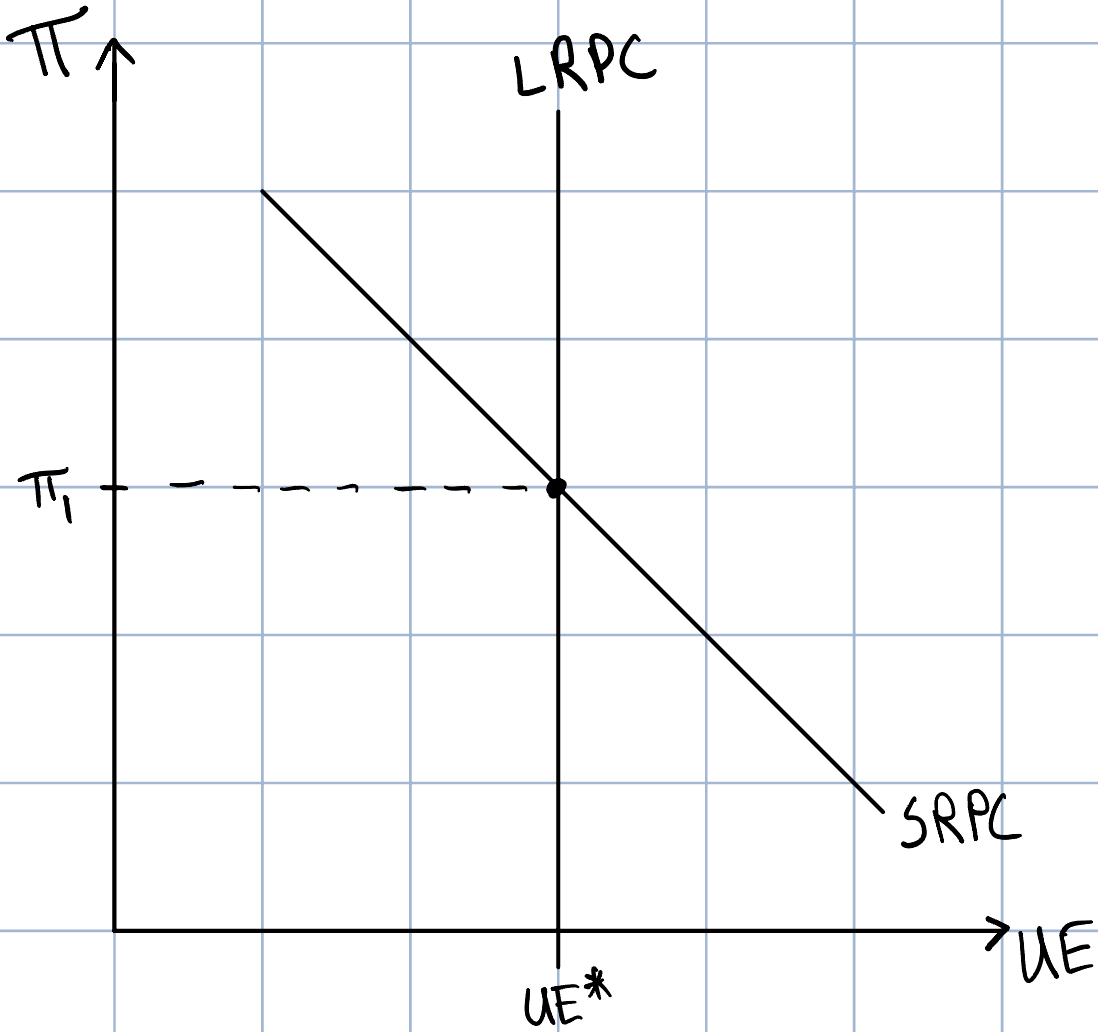
\includegraphics[width = 0.4\textwidth]{paa4a}
		\end{center}
	
	\item If the AD curve shifts left, the price level and output fall. As a result, inflation decreases, and the unemployment rate increases. That causes a movement down and to the left along the short-run Phillips curve.
	
	If the Fed undertook expansionary monetary policy, it could shift the AD curve back to its original position. Doing so would return the economy to its original inflation rate and unemployment rate.
	
		\begin{center}
		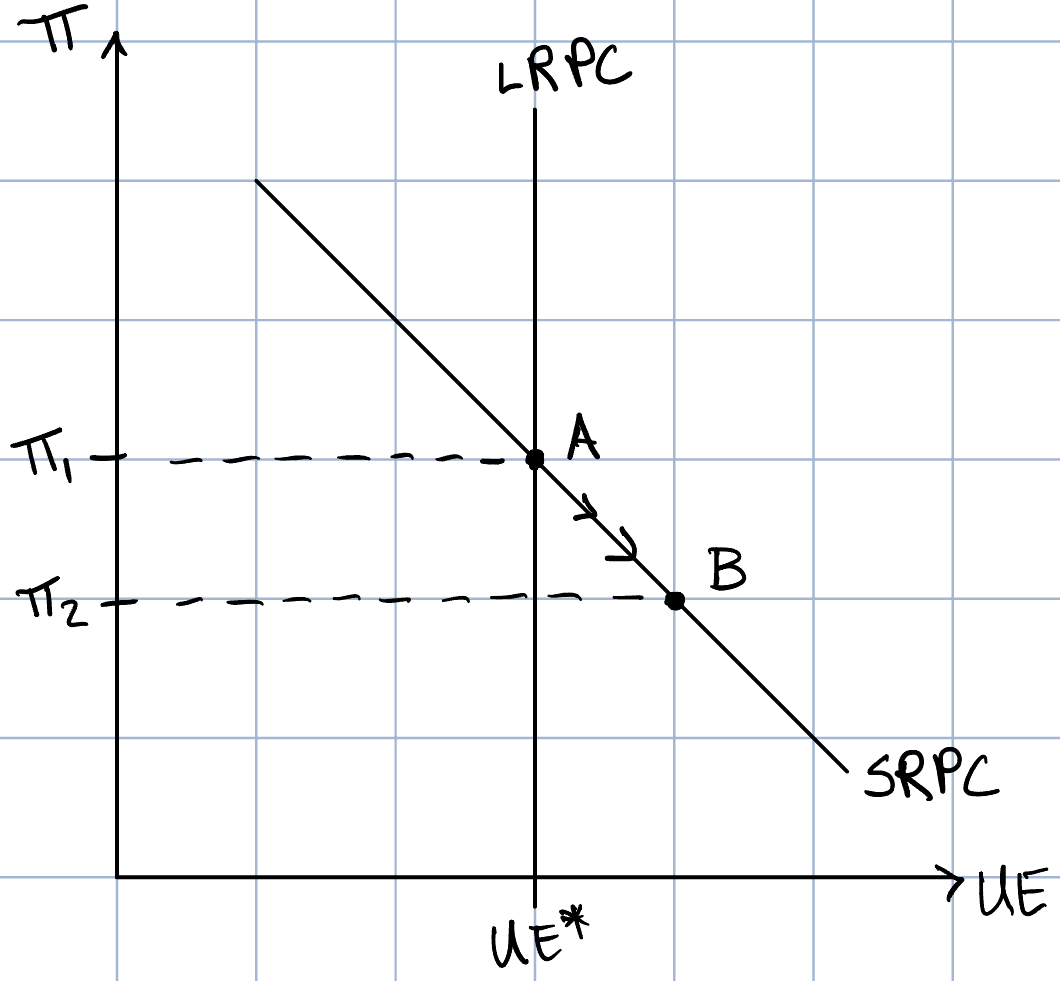
\includegraphics[width = 0.4\textwidth]{paa4b}
		\end{center}
		
	\item An increase in oil prices is a negative supply shock. If the SRAS curve shifts left, the Phillips curve shifts right.
	
		\begin{center}
		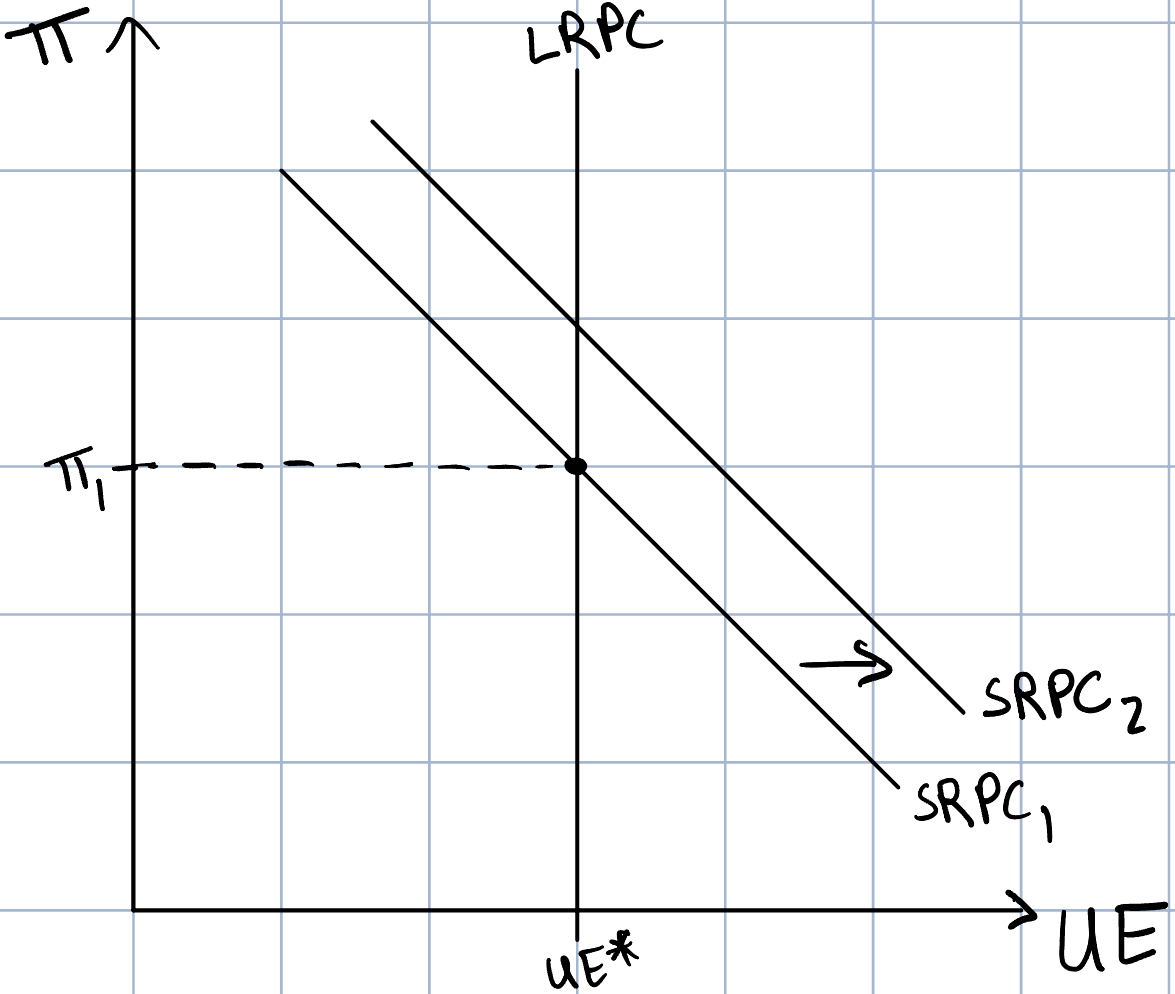
\includegraphics[width = 0.4\textwidth]{paa4c1}
		\end{center}
		
	If the Fed undertakes expansionary monetary policy, it can return the economy to its original unemployment rate but it can't return it to its original inflation rate. Expansionary monetary policy will shift AD to the right which will restore full-employment output but increase inflation. 
	
		\begin{center}
		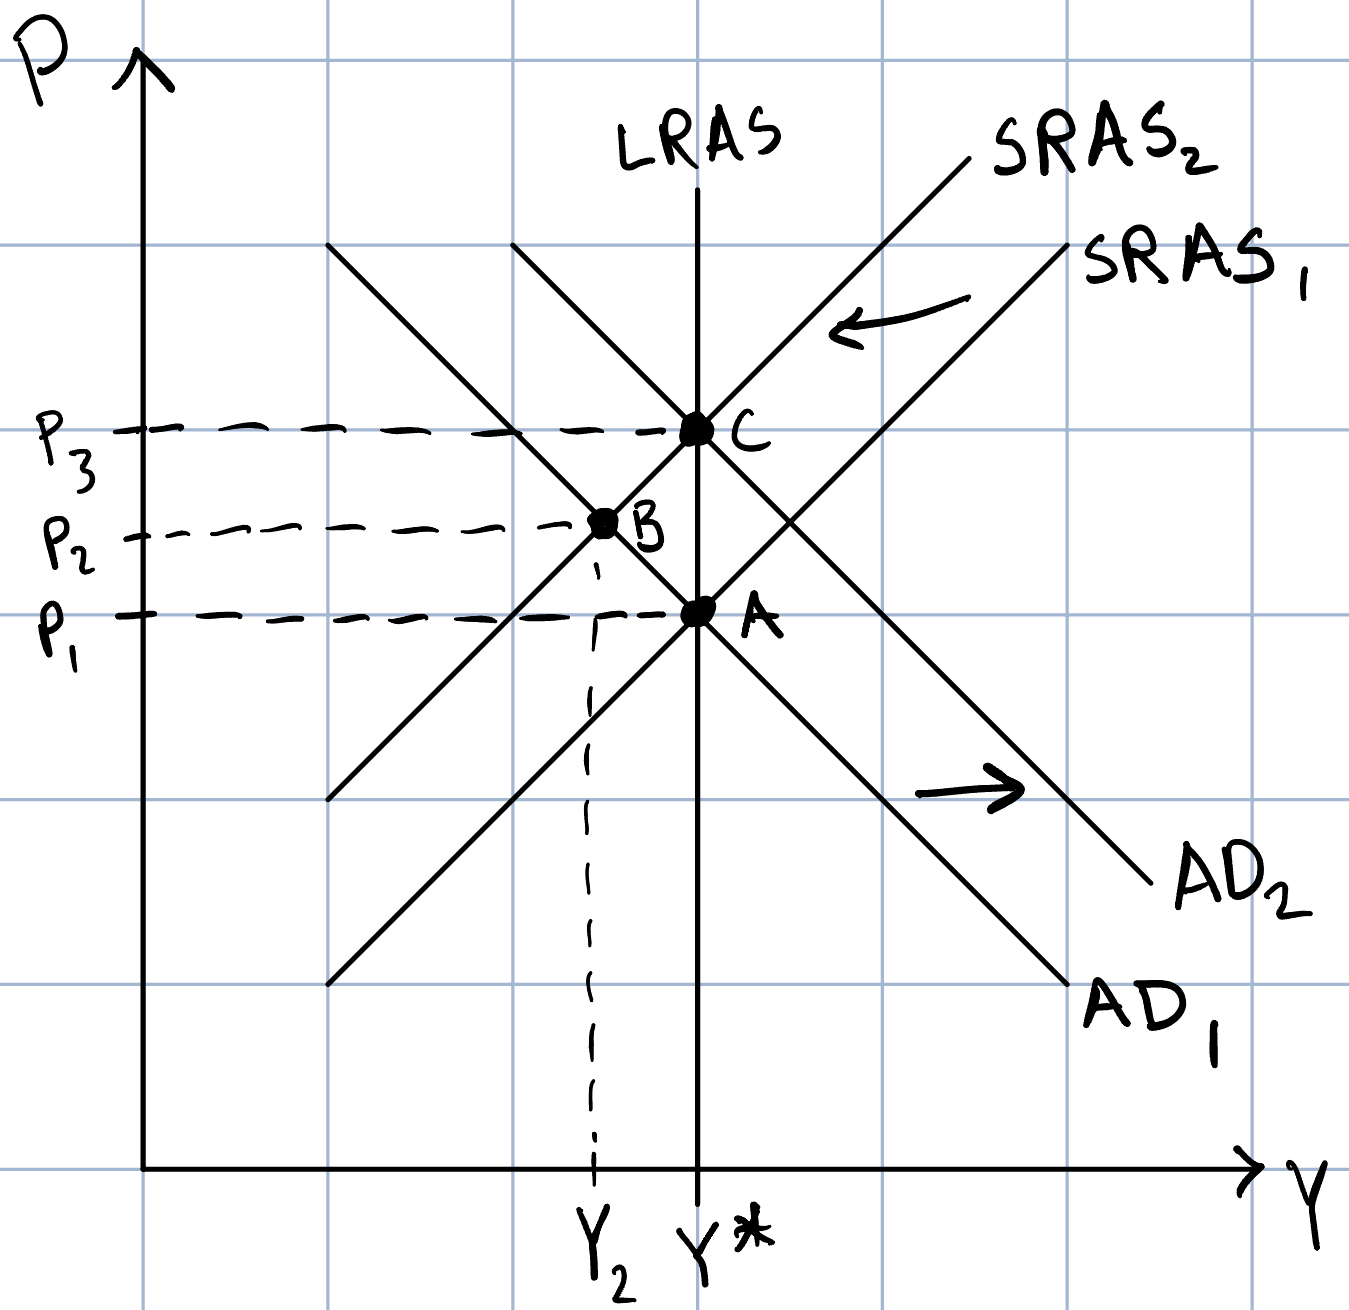
\includegraphics[width = 0.4\textwidth]{paa4c2}
		\end{center}
	
	\end{enumerate}
	
\item Milton is more likely to favor the proposed change. When the Fed slows the rate of money growth, the economy will experience a period of low output and high unemployment while disinflating.

	\begin{center}
	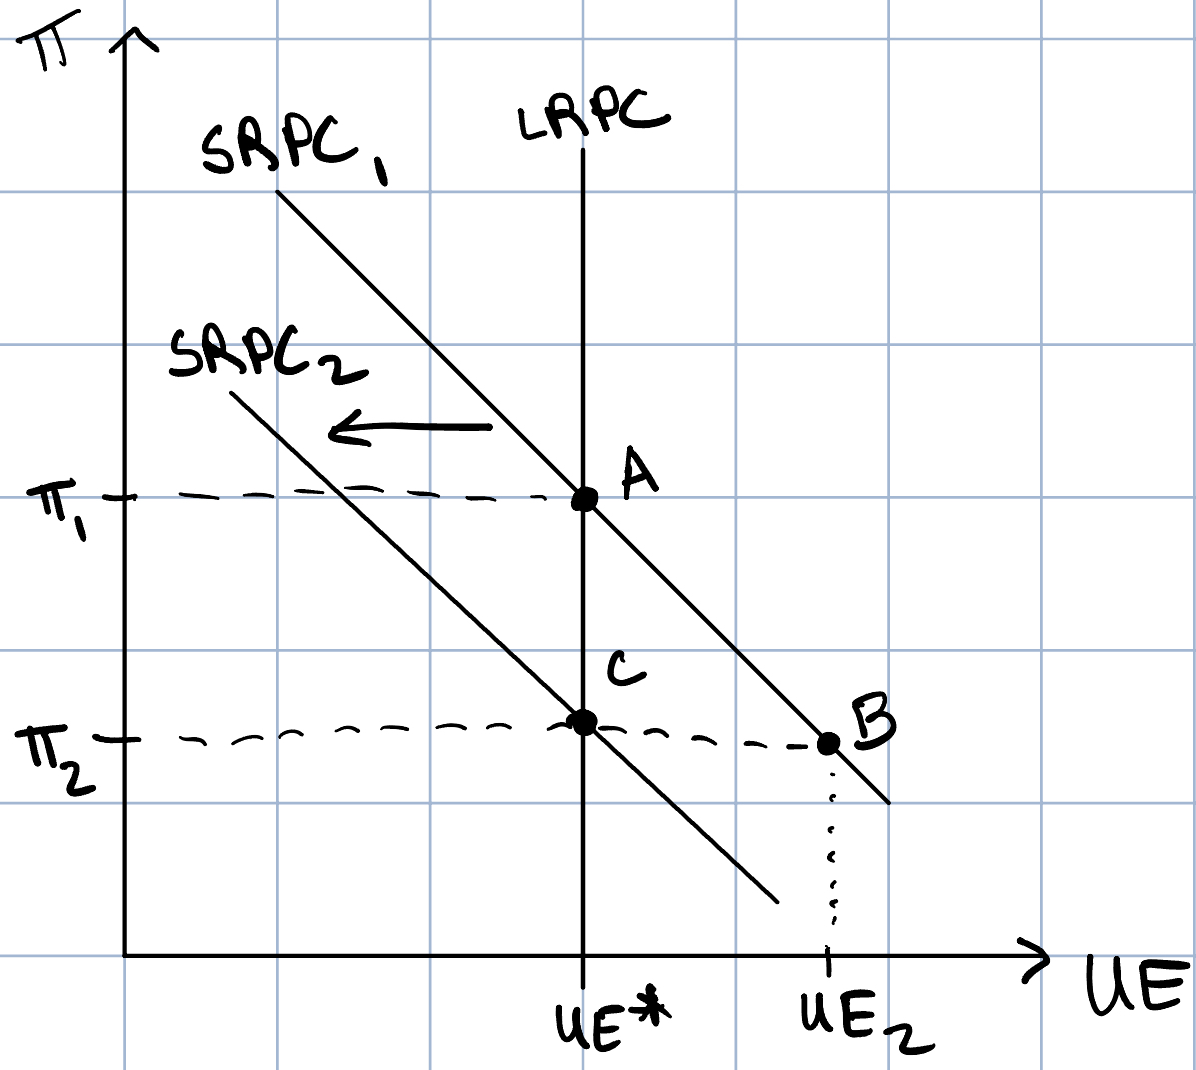
\includegraphics[width = 0.4\textwidth]{paa5}
	\end{center}

If people change their expectations quickly, that period will be briefer because the Phillips curve will shift left more quickly.

\end{enumerate}

\end{document}